% Options for packages loaded elsewhere
\PassOptionsToPackage{unicode}{hyperref}
\PassOptionsToPackage{hyphens}{url}
\PassOptionsToPackage{dvipsnames,svgnames,x11names}{xcolor}
%
\documentclass[
  11pt,
  a4paper,
  openany]{book}

\usepackage{amsmath,amssymb}
\usepackage{iftex}
\ifPDFTeX
  \usepackage[T1]{fontenc}
  \usepackage[utf8]{inputenc}
  \usepackage{textcomp} % provide euro and other symbols
\else % if luatex or xetex
  \usepackage{unicode-math}
  \defaultfontfeatures{Scale=MatchLowercase}
  \defaultfontfeatures[\rmfamily]{Ligatures=TeX,Scale=1}
\fi
\usepackage{lmodern}
\ifPDFTeX\else  
    % xetex/luatex font selection
\fi
% Use upquote if available, for straight quotes in verbatim environments
\IfFileExists{upquote.sty}{\usepackage{upquote}}{}
\IfFileExists{microtype.sty}{% use microtype if available
  \usepackage[]{microtype}
  \UseMicrotypeSet[protrusion]{basicmath} % disable protrusion for tt fonts
}{}
\makeatletter
\@ifundefined{KOMAClassName}{% if non-KOMA class
  \IfFileExists{parskip.sty}{%
    \usepackage{parskip}
  }{% else
    \setlength{\parindent}{0pt}
    \setlength{\parskip}{6pt plus 2pt minus 1pt}}
}{% if KOMA class
  \KOMAoptions{parskip=half}}
\makeatother
\usepackage{xcolor}
\usepackage[top=35mm,right=25mm,bottom=35mm,left=25mm,heightrounded]{geometry}
\setlength{\emergencystretch}{3em} % prevent overfull lines
\setcounter{secnumdepth}{5}
% Make \paragraph and \subparagraph free-standing
\ifx\paragraph\undefined\else
  \let\oldparagraph\paragraph
  \renewcommand{\paragraph}[1]{\oldparagraph{#1}\mbox{}}
\fi
\ifx\subparagraph\undefined\else
  \let\oldsubparagraph\subparagraph
  \renewcommand{\subparagraph}[1]{\oldsubparagraph{#1}\mbox{}}
\fi
\pagestyle{plain}


\providecommand{\tightlist}{%
  \setlength{\itemsep}{0pt}\setlength{\parskip}{0pt}}\usepackage{longtable,booktabs,array}
\usepackage{calc} % for calculating minipage widths
% Correct order of tables after \paragraph or \subparagraph
\usepackage{etoolbox}
\makeatletter
\patchcmd\longtable{\par}{\if@noskipsec\mbox{}\fi\par}{}{}
\makeatother
% Allow footnotes in longtable head/foot
\IfFileExists{footnotehyper.sty}{\usepackage{footnotehyper}}{\usepackage{footnote}}
\makesavenoteenv{longtable}
\usepackage{graphicx}
\makeatletter
\def\maxwidth{\ifdim\Gin@nat@width>\linewidth\linewidth\else\Gin@nat@width\fi}
\def\maxheight{\ifdim\Gin@nat@height>\textheight\textheight\else\Gin@nat@height\fi}
\makeatother
% Scale images if necessary, so that they will not overflow the page
% margins by default, and it is still possible to overwrite the defaults
% using explicit options in \includegraphics[width, height, ...]{}
\setkeys{Gin}{width=\maxwidth,height=\maxheight,keepaspectratio}
% Set default figure placement to htbp
\makeatletter
\def\fps@figure{htbp}
\makeatother

\usepackage{hyphenat}
\usepackage{graphicx}
\usepackage{wallpaper} % for the background image on title page
\usepackage{geometry} % for margins
\usepackage{babel}
\usepackage{libertine}
\usepackage[most]{tcolorbox}
\usepackage{setspace}
\usepackage{parskip}
\usepackage{contour}

\onehalfspacing % line spacing
\setlength{\parskip}{1.5em}
\setlength\parindent{0pt}
\makeatletter
\@ifpackageloaded{bookmark}{}{\usepackage{bookmark}}
\makeatother
\makeatletter
\@ifpackageloaded{caption}{}{\usepackage{caption}}
\AtBeginDocument{%
\ifdefined\contentsname
  \renewcommand*\contentsname{Table of contents}
\else
  \newcommand\contentsname{Table of contents}
\fi
\ifdefined\listfigurename
  \renewcommand*\listfigurename{List of Figures}
\else
  \newcommand\listfigurename{List of Figures}
\fi
\ifdefined\listtablename
  \renewcommand*\listtablename{List of Tables}
\else
  \newcommand\listtablename{List of Tables}
\fi
\ifdefined\figurename
  \renewcommand*\figurename{Figure}
\else
  \newcommand\figurename{Figure}
\fi
\ifdefined\tablename
  \renewcommand*\tablename{Table}
\else
  \newcommand\tablename{Table}
\fi
}
\@ifpackageloaded{float}{}{\usepackage{float}}
\floatstyle{ruled}
\@ifundefined{c@chapter}{\newfloat{codelisting}{h}{lop}}{\newfloat{codelisting}{h}{lop}[chapter]}
\floatname{codelisting}{Listing}
\newcommand*\listoflistings{\listof{codelisting}{List of Listings}}
\makeatother
\makeatletter
\makeatother
\makeatletter
\@ifpackageloaded{caption}{}{\usepackage{caption}}
\@ifpackageloaded{subcaption}{}{\usepackage{subcaption}}
\makeatother
\ifLuaTeX
  \usepackage{selnolig}  % disable illegal ligatures
\fi
\usepackage{bookmark}

\IfFileExists{xurl.sty}{\usepackage{xurl}}{} % add URL line breaks if available
\urlstyle{same} % disable monospaced font for URLs
\hypersetup{
  pdftitle={Die barocken Schloss- und Gartenveduten},
  pdfauthor={Jane Doe; Maxine Mustermann; Neptune III.},
  colorlinks=true,
  linkcolor={Maroon},
  filecolor={Maroon},
  citecolor={Blue},
  urlcolor={cyan},
  pdfcreator={LaTeX via pandoc}}

\title{Die barocken Schloss- und Gartenveduten}
\usepackage{etoolbox}
\makeatletter
\providecommand{\subtitle}[1]{% add subtitle to \maketitle
  \apptocmd{\@title}{\par {\large #1 \par}}{}{}
}
\makeatother
\subtitle{Versuch eines PDF-Buchs}
\author{Jane Doe \and Maxine Mustermann \and Neptune III.}
\date{2024-06-15}

\begin{document}
  \begin{frontmatter}
  \begin{titlepage}
  %  SOURCE: https://github.com/nmfs-opensci/quarto_titlepages_v1/tree/main

  % This is a combination of Pandoc templating and LaTeX
  % Pandoc templating https://pandoc.org/MANUAL.html#templates

  \tcbset{ % parameters for text background 
      frame code={},
      left=0pt, % margins
      right=0pt,
      top=0pt,
      bottom=0pt,
      colback=gray!10!black, % box color
      width=\dimexpr\textwidth\relax, 
      boxsep=15pt, % spacing between boxes
      arc=0pt, % no rounded edges
      opacityback=0.35, % translucent-ish background
      fontupper=\color{white}, % fontcolor
      fontlower=\color{white}
      }

  % background image
    \ThisULCornerWallPaper{1}{images/cover.jpg}

  \begin{tcolorbox}


  \centering

  % Title and subtitle
  {\Huge\bfseries\nohyphens{Die barocken Schloss- und
  Gartenveduten}}\\[1\baselineskip]
    {\huge{Versuch eines PDF-Buchs}}\\[4\baselineskip]

  \end{tcolorbox}

  \bigbreak

  % Authors
  \begin{tcolorbox}

        {\large{Jane Doe}}{\textsuperscript{1}}%
    %
    \textsuperscript{,}%
    {\textsuperscript{*}}%
    %
    , 
        {\large{Maxine Mustermann}}{\textsuperscript{2}}%
    %
    \textsuperscript{,}%
    {\textsuperscript{*}}%
    %
      %
      { and \large{Neptune III.}}%
    {\textsuperscript{3}}%
    %
    
    
  %%%%%% Affiliations
  \vspace{2\baselineskip} 

  \hangindent=1em
  \hangafter=1
  %
  {1}.~{Minnesota Department of Natural Resources}%
  %
  %
  , %
  {500 Lafayette Road Saint Paul, MN 55155}%
  %
  \par\hangindent=1em\hangafter=1%
  %
  {2}.~{University of Minnesota}%
  %
  , %
  {Department of Mathematics}%
  %
  %
  \par\hangindent=1em\hangafter=1%
  %
  {3}.~{University of Somewhere}%
  %
  , %
  {Department of Marine Biology}%
  %
  %


  %%%%%% Correspondence
  \vspace{1\baselineskip} 

  * \textit{Correspondence:}~Jane Doe~jd@college.edu\newline
  * \textit{Correspondence:}~Maxine Mustermann~mm@um-mail.edu\newline

  \end{tcolorbox}


  %use \vfill instead to get the space to fill flexibly	
  %\vspace{0.25\textheight} % Whitespace between the title block and the publisher

  \vfill

  % Whitespace between the title block and the tagline
  \vspace{1\baselineskip} 

  \begin{tcolorbox}
  \centering

  %%%%%% Tagline at bottom
  {
    TIB\\
    Open Science Lab
  }
  \end{tcolorbox}
  
  \end{titlepage}
  \end{frontmatter}

{\let\newpage\relax}
\renewcommand*\contentsname{Inhaltsverzeichnis}
{
\hypersetup{linkcolor=}
\setcounter{tocdepth}{2}
\tableofcontents
}
\mainmatter
\bookmarksetup{startatroot}

\chapter*{Katalog zur Ausstellung: Die barocken Schloss- und
Gartenveduten}\label{katalog-zur-ausstellung-die-barocken-schloss--und-gartenveduten}
\addcontentsline{toc}{chapter}{Katalog zur Ausstellung: Die barocken
Schloss- und Gartenveduten}

\markboth{Katalog zur Ausstellung: Die barocken Schloss- und
Gartenveduten}{Katalog zur Ausstellung: Die barocken Schloss- und
Gartenveduten}

Ein Katalog mit Kunstwerken aus der CbDD-Sammlung. Textteil:
\href{https://www.deckenmalerei.eu/42d06165-58e7-4653-bfe4-3d5f7091fc33\#6e73f774-4b7f-4e37-937b-e11cc35c5bc8}{6e73f774-4b7f-4e37-937b-e11cc35c5bc8}

Die barocken Schloss- und Gartenveduten {[}Sammlung{]}

This work is licensed under a Creative Commons
Attribution-NonCommercial-NoDerivs 4.0 International License.

\bookmarksetup{startatroot}

\chapter{Die barocken Schloss- und
Gartenveduten}\label{die-barocken-schloss--und-gartenveduten}

Wikibase link:
\url{https://computational-publishing-service.wikibase.cloud/entity/Q252}

Kurator: Seeger, Ulrike

\subsection{Belagerung I: „Vestung Tottis, wie die von den Christen bei
der Nacht erobert worden,
1590``}\label{belagerung-i-vestung-tottis-wie-die-von-den-christen-bei-der-nacht-erobert-worden-1590}

Breites Format. Vorne rechts ins Bild hineinreitende Reiter mit großen
Fahnen. Im Hintergrund die ungarische Festung Totis (Tata) nach dem
Vorbild von Sibmachers Kupferstich, der allerdings eine Eroberung durch
die Christen aus dem Jahr 1597 wiedergibt. Die sehr dunkle Szenerie wird
von zwei Laternen spärlich erleuchtet. Da Totis nicht 1590, sondern 1597
und 1598 durch die Christen erobert wurde, und zudem zu den zeitlich als
nächste dargestellten Belagerungen eine Zeitspanne von vier Jahren
liegt, kann es gut sein, dass der Jahreszahl 1590 ein Versehen zugrunde
liegt.

Wikibase link:
\url{https://computational-publishing-service.wikibase.cloud/entity/Q253}

Kurator: Seeger, Ulrike

\subsection{Belagerung II: „Vestung Gran wie die von Christen belegert
gewesen.
1594``}\label{belagerung-ii-vestung-gran-wie-die-von-christen-belegert-gewesen.-1594}

Schmales Format. Vorne links ein Hellebardier mit einem Knecht, der mit
schwarzen Kugeln als Munition hantiert. Von rechts kommt dynamisch ein
Reiter mit rotem Mantel, schwarzem Zylinder und möglicherweise einer
Trompete im Arm ins Bild geritten. Da an der versuchten Einnahme von
Gran (Eszergom) im Jahr 1594 Graf Georg Friedrich, der älteste Sohn von
Graf Wolfgang II., als kaiserlicher Obrist beteiligt war,{[}1{]} darf
man den Reiter im roten Mantel vermutlich mit diesem identifizieren.
Sein Gesicht folgt mit hellem Teint, roten Bäckchen, hoher Stirn,
Schnauzbart und fein geschwungenen Augenbrauen dem des Grafen Wolfgang
auf den Deckengemälden des Rittersaals mit dem Unterschied, dass es von
dunkelbraunem Haar gerahmt wird.

Im Mittelgrund blickt man auf das Feldlager der kaiserlichen Armee. Von
einer Verschanzung in den Donauauen wird am gegenüberliegenden Ufer die
Wasserstadt von Gran beschossen. Darüber liegt die Festung Gran mit der
Doppelturmfassade der Kathedrale. Mehrere Minarette deuten die türkische
Herrschaft an. Die Ansicht folgt nicht dem Kupferstich von Sibmacher,
der Gran von einem anderen Blickwinkel und zudem summarischer zeigt.
Ohnehin hat Sibmacher nicht die Belagerung des Jahres 1594, sondern die
des Jahres 1595 dargestellt. Da Georg Friedrich an dem Ereignis 1594
beteiligt war, dürfte die Weikersheimer Darstellung auf Flugblätter oder
bebilderte Zeitungsberichte zurückgehen, die es mannigfach zu den
Ereignissen des Langen Türkenkriegs gab. Der von links mit einer Drehung
ins Bild hineinreitende Reiter hat sein Vorbild in einem Stich von
Stradanus zur Wolfsjagd (Nachdruck Olms, Tf. 20).

{[}1{]} Trentin-Meyer, Georg Friedrich von Hohenlohe, 2019, S. 90.

Wikibase link:
\url{https://computational-publishing-service.wikibase.cloud/entity/Q254}

Kurator: Seeger, Ulrike

\subsection{Belagerung III: „Vestung Raab, wie die vom Türcken belegert
gewesen. A{[}nn{]}o
1594''}\label{belagerung-iii-vestung-raab-wie-die-vom-tuxfcrcken-belegert-gewesen.-anno-1594}

Breites Format. Von rechts kommen türkische Reiter ins Bild. Im
Mittelgrund ist am gegenüberliegenden Ufer der Donau die quadratische
Festung Raab (Győr) zu erkennen. Ihre Eckbastionen und die Bastion an
einer links zusätzlich stumpfwinkelig vorstoßenden Ecke sind mit Kanonen
besetzt. Die vom Feldlager der Türken umzingelte Festung wird heftig
beschossen. Im Vordergrund spielt sich am linken unteren Bildrand ein
Nahkampf zwischen Christen und Türken ab, der sich neben zwei
Transportkutschen entzündet hat. Die Darstellung der Festung und der
Kampfhandlungen folgt getreu der Vorlage bei Ortelius.

Wikibase link:
\url{https://computational-publishing-service.wikibase.cloud/entity/Q255}

Kurator: Seeger, Ulrike

\subsection{Belagerung IV: „Vestung Comorna wie die vom Türckn belegert
gewe{[}sen{]}
1594``}\label{belagerung-iv-vestung-comorna-wie-die-vom-tuxfcrckn-belegert-gewesen-1594}

Breites Format. Von links kommen türkische Reiter ins Bild, von denen
ein blau gekleideter Frontmann eine lange Lanze mit blauer Fahne
dynamisch diagonal ins Bild stößt. Rechts unten knien vor türkischen
Zelten zwei Dromedare. Den Höcker des vorderen Dromedars bedeckt ein
blaues Tuch mit aufgesticktem Sonnensymbol. Der Mittelgrund ist durch
den Verlauf der Donau zweigeteilt. Am Ufer im Vordergrund formiert sich
ein türkisches Heer. Auf der gegenüberliegenden Seite liegt die von den
Christen gehaltene Festung von Komorn (Komárom). Sie überstand die
Belagerung unversehrt, während die hinter der Festung anschließende
Stadt in Flammen steht.

Die Festung Komorn besetzte eine Landspitze an der Mündung der Waag in
die Donau. Sie wurde von dem kaiserlichen Festungsbaumeister Pietro
Ferrabosco unterstützt durch Daniel Specklin auf einem dreieckigen
Grundriss angelegt. Die türkische Belagerung 1594 überstand sie
unversehrt. In der Folgezeit wurde sie verstärkt und weiterhin nicht
eingenommen. Mit der Darstellung der Festung und der brennenden Stadt
Komorn folgte Katzenberger treu dem Vorbild Sibmachers. Die Anregung zu
den beiden Dromedaren im Vordergrund erhielt er ebenfalls von Sibmacher,
der die Dromedare als Reittiere der Osmanen im Vordergrund allerdings
nur klein darstellte.

Wikibase link:
\url{https://computational-publishing-service.wikibase.cloud/entity/Q256}

Kurator: Seeger, Ulrike

\subsection{Belagerung V: „Vestung Gran wie die von den Christen wider
erobert worden. A{[}nn{]}o
1595.``}\label{belagerung-v-vestung-gran-wie-die-von-den-christen-wider-erobert-worden.-anno-1595.}

Breites Format. Im Vordergrund links beugt sich eine Rückenfigur nach
vorne, sodass sie dem Betrachter den Hintern zeigt. Am rechten unteren
Bildrand steht die Halbfigur eines Höflings mit Flinte und braunem
Pferd. Dem Gesicht nach zu urteilen, handelt es sich um einen der Söhne
von Graf Wolfgang. Im Mittelgrund ist eine Schlacht mit türkischen
Reitern mit langen Lanzen zu sehen. Den Hintergrund bildet eine im
Dunkeln liegende Hügellandschaft, in der auf einem Berg die Festung Gran
(Győr), am Ufer der Donau die zugehörige Wasserstadt und vor allem die
ebenfalls befestigte Ratzenstadt (Rácvázószöveg) gut zu erkennen sind.
Die Landschaft folgt treu der Vorlage bei Ortelius.

Die Fahnen lassen den Stand der Eroberung erkennen, was sich dem
heutigen Betrachter nur noch mithilfe der Erläuterungen auf dem
Kupferstich bei Ortelius erschließt. Über der Festung Gran, die laut
Ortelius am 3. August eingenommen wurde, weht klein noch die türkische
Fahne mit einer gelben Sonne auf rotem Grund. Über der Ratzenstadt, die
im Juli als erstes erobert wurde, weht groß die Fahne der Kaiserlichen
mit gewelltem weißem Andreaskreuz auf rotem Grund. Die Wasserstadt, über
der bei Katzenberger die kaiserliche Fahne mit dem Reichsadler auf
goldenem Grund steht, wurde laut Ortelius Ende August erobert, sodass
mit Ende August der zur Darstellung gelangte Zeitpunkt getroffen sein
dürfte.

Wikibase link:
\url{https://computational-publishing-service.wikibase.cloud/entity/Q257}

Kurator: Seeger, Ulrike

\subsection{Belagerung VI: ``Vestung Vizzegrad wie die von Christen
belegert gewesen Anno
1595``}\label{belagerung-vi-vestung-vizzegrad-wie-die-von-christen-belegert-gewesen-anno-1595}

Breites Format. Im Vordergrund stehen in der linken Bildhälfte zwei
prächtig gekleidete Offiziere, einer als Rückenfigur mit Rüstung und
Federbusch, einer mit grau schimmerndem Gewand und auffälligem Helm.
Derjenige im grauen Gewand wendet den Blick dem Betrachter zu. Da an der
Belagerung der Neffe von Papst Clemens VIII., Giovanni Francesco
Aldobrandini, beteiligt war, könnte es sich um diesen und einen
Begleiter handeln. Rechts vorne machen sich Männer an Kanonen zu
schaffen. Im Hintergrund erhebt sich charakteristisch auf einem
kegelförmigen Berg am Ufer der Donau die Zitadelle von Visegrád. Sie
beherrscht einen großen natürlichen Hafen mit zahlreichen
Transportschiffen. Das Gemälde lebt stimmungsvoll von silbrigen
Grautönen, aus denen vereinzelt rote Fahnen und andere Details rot
herausleuchten.

Wikibase link:
\url{https://computational-publishing-service.wikibase.cloud/entity/Q258}

Kurator: Seeger, Ulrike

\subsection{Belagerung VII: „Statt Waitzen wie die von vom Türcken
belegert gewesen
1597``}\label{belagerung-vii-statt-waitzen-wie-die-von-vom-tuxfcrcken-belegert-gewesen-1597}

Schmales Format. Rechts im Vordergrund reitet ein Türke mit Turban und
Streitkolben frontal auf den Betrachter zu. Links unter ihm steht ein
türkisches Zelt. Im Hintergrund liegt an der Donau Waitzen (Vác), das
sich aus einer befestigten Stadt und einem befestigten Kloster
zusammensetzt. In der Stadt, an deren Rand sich eine Moschee befindet,
brennen mehrere Häuser. Verglichen mit dem Kupferstich bei Ortelius sind
Stadt und Kloster seitenverkehrt dargestellt.

Wikibase link:
\url{https://computational-publishing-service.wikibase.cloud/entity/Q259}

Kurator: Seeger, Ulrike

\subsection{Belagerung VIII: „Vestung Raab, die Christen beÿ der Nacht
wider erobert. A{[}nn{]}o
1598''}\label{belagerung-viii-vestung-raab-die-christen-beuxff-der-nacht-wider-erobert.-anno-1598}

Schmales Format. Katzenberger hat die Belagerung effektvoll als
Nachtbild vergegenwärtigt. Vorne rechts stehen zwei Wachsoldaten, deren
Rüstungen und Gewänder im Schein der Laternen aufleuchten. Im
Hintergrund liegt die Festung Raab (Győr), an deren Bastionen sich an
zwei Stellen große Explosionen ereignen. Katzenberger hat sie mitsamt
den Feuerherden exakt von Sibmacher übernommen.

Wikibase link:
\url{https://computational-publishing-service.wikibase.cloud/entity/Q260}

Kurator: Seeger, Ulrike

\subsection{Belagerung IX: „Hauptstatt Offen. wie die von Christen
belegert gewesen.
1598.``}\label{belagerung-ix-hauptstatt-offen.-wie-die-von-christen-belegert-gewesen.-1598.}

Breites Format. Im Vordergrund steht eine große Kanone, die von Pferden
nach links aus dem Bild gezogen wird. Auf der Kanone sitzt der Kutscher
mit Pelzmütze, mongolisch anmutendem Bart und rotem Mantel. Er schwingt
eine lange Peitsche. Am rechten Bildrand steht ein junger, ebenfalls
mongolisch aussehender Mann in einem hellen Wams. Hinter der fahrenden
Kanone rennt ein Jagdhund her.

Im Hintergrund erstreckt sich Ofen (Óbuda, heute Buda als Stadtteil von
Budapest) als prächtige Stadt mit hoher Stadtmauer, einem Schloss,
zahlreichen Kirchen und Minaretten sowie außerhalb der Mauern einem
Lustgarten mit Pavillon. Der Lustgarten ist dem Schloss, auf dem bei
Ortelius eine türkische Fahne weht, unmittelbar vorgelagert. Im
Mittelgrund liegt ebenfalls außerhalb der Stadtmauern ein türkischer
Friedhof mit zahlreichen Grabsteinen und einem runden gedrungenen Turm
in der Mitte. Katzenberger hat die Stadtansicht mitsamt der Schilderung
des Lustgartens und des Friedhofs von Sibmacher übernommen.

Wikibase link:
\url{https://computational-publishing-service.wikibase.cloud/entity/Q261}

Kurator: Seeger, Ulrike

\subsection{Belagerung X: „Hauptstatt Offen, wie die von Christen
belegert gewesen. Anno
1603``}\label{belagerung-x-hauptstatt-offen-wie-die-von-christen-belegert-gewesen.-anno-1603}

Breites Format. Vorne rechts reitet auf einem grauen Pferd ein
gerüsteter kaiserlicher Heerführer mit weißem Federbusch ins Bild.
Seinem Gesichtsschnitt und dem blonden Bart zufolge handelt es sich um
einen Sohn von Graf Wolfgang. Vor ihm läuft ein Knappe mit prächtigem
roten Mantel, rotem Federbusch und einem Gewehr über der Schulter. Er
weist ihm den Weg zum Feldlager. Hinter dem Feldlager stehen auf der
anderen Seite eines Donauzuflusses Truppen in Aufstellung. An einer
Verschanzung werden Kanonen gezündet. Der Geländezipfel zwischen Donau
und Zufluss ist mit einer dreieckigen Festung besetzt, zu der sich eine
Schiffbrücke spannt. Die in der vorangegangenen Belagerung von Ofen aus
dem Jahr 1598 prächtig geschilderte Stadt Ofen (Óbuda, heute Buda als
Stadtteil von Budapest) befindet sich auf dem Gemälde angeschnitten am
linken Bildrand. Sie ist an den vorgelagerten Donauinseln zu erkennen,
auf die weitere Schiffbrücken führen.

Katzenberger konnte für die Belagerung von 1703 nicht mehr auf Ortelius
zurückgreifen, dessen Werk 1702 erschien. Vermutlich orientierte er sich
an Schilderungen des Sohnes und übernahm die Flussmündung mit der
dreieckigen Festung aus der Darstellung einer anderen Belagerung, da sie
sich auf Karten der Donau bei Buda nicht finden lässt.

Wikibase link:
\url{https://computational-publishing-service.wikibase.cloud/entity/Q262}

Kurator: Seeger, Ulrike

\subsection{Belagerung XI: „Hauptstatt Offen, wie die von Christn
belegert gewesen, ein Schärmützell. darbei geschehen.
1603``}\label{belagerung-xi-hauptstatt-offen-wie-die-von-christn-belegert-gewesen-ein-schuxe4rmuxfctzell.-darbei-geschehen.-1603}

Schmales Format. Im Vordergrund stehen zwei von hinten gezeigte Pferde,
die mit Kanonenrohren, Wagenrädern und Pauken beladen sind. Neben ihnen
geht rechts ein schwarz gekleideter Mann mit grauem Schlapphut. Im
Hintergrund zieht sich in starker Aufsicht wie auf einer Landkarte die
Donau bei Ofen (Óbuda) und Pest mit den Donauinseln hin. Hinter dem
Fluss hat Katzenberger klein das Scharmützel dargestellt. Es spielt sich
auf offenem Terrain ab vor einem Zeltlager und einem Hügel, von dem aus
Kanonen gezündet werden. Links oben im Bild ist die breit gelagerte
befestigte Stadt Ofen zu sehen.

Die Belagerung von 1603 war nicht mehr in der 1602 erschienenen Chronik
von Ortelius enthalten. Vermutlich wurde sie in den Zyklus aufgenommen,
weil ein Sohn Graf Wolfgangs daran beteiligt war. Das Gemälde stammt dem
Aufbau und der Malweise zufolge von Katzenberger. In Ermangelung einer
Vorlage behalf er sich für den Verlauf der Donau einer Landkarte. Die
Festungen im Mittel- und Hintergrund konnte er aus den vorangegangenen
Belagerungen entwickeln.

Wikibase link:
\url{https://computational-publishing-service.wikibase.cloud/entity/Q263}

Kurator: Seeger, Ulrike

\subsection{Belagerung XII: „Vestung Gran wie die vom Türcken belegert
gewesen A{[}nn{]}o
1604``}\label{belagerung-xii-vestung-gran-wie-die-vom-tuxfcrcken-belegert-gewesen-anno-1604}

Breites Format. Im Vordergrund ein ausnahmsweise mit seiner Breitseite
vorgestelltes braunes Pferd, dessen Reiter sich dem Betrachter frontal
zuwendet. Der Reiter trägt keine Rüstung, sondern ein wollweißes Wams,
einen rotsamtenen Rock mit Goldbesatz und über der Brust eine voluminöse
rote Schärpe. Die Schärpe wird von einem auffälligen Schmuckring
zusammengehalten, ihr loses Ende flattert im Wind zusammen mit dem
Schweif des Pferdes. Der Reiter trägt einen breitkrempigen schwarzen Hut
mit Goldrand und rotem Federbusch. Bei dem Dargestellten handelt es sich
um Graf Ludwig Kasimir, der jüngste Sohn von Graf Wolfgang, der bei der
Belagerung von Gran (Eszergom) im Jahr 1604 sein Leben ließ. Sein
ernstes hochovales Gesicht mit blonden Haaren und schwachem Bartwuchs
folgt dem Gesichtstyp, der auf den Deckengemälden des Rittersaals
mehrfach Graf Wolfgang zuzuordnen war.

Am unteren Bildrand ist deutlich kleiner und einer anderen
Realitätsebene angehörend eine höfisch gekleidete Frau zu sehen, der von
einem Soldaten der Weg gewiesen wird. Es könnte sich hierbei um die
Mutter des kinderlos verstorbenen Sohns, Magdalena von
Nassau-Katzenelnbogen handeln. Sie hält in der rechten Hand einen
Stieglitz, der wegen seines blutroten Kopfgefieders und goldener
Flugfedern als Symbol des Opfertods Christi galt.{[}1{]} Der schwarze
Salamander auf ihrer linken Brust war ein geläufiges Sinnbild der
Auferstehung Christi und brachte die Hoffnung auf ein Leben nach dem Tod
zum Ausdruck. Auf ihrer Schulter sitzt ein Äffchen, das an die Eitelkeit
des Menschen gemahnen könnte. Hinter dem Paar geht ein Knecht mit
traurigem Gesichtsausdruck.

Im Hintergrund verläuft als großzügig geschwungener Bogen die Donau, an
deren Ufer eine ringförmig mehrfach befestigte Zitadelle und mehrere
befestigte Höhenzüge zu sehen sind. Der Blickwinkel auf den Fluss ist
zwar sehr exponiert, doch ist er -- im Unterschied zur Belagerung von
Ofen 1603 -- nicht minutiös einer Landkarte entnommen. Der Duktus der
Landschaft, des Himmels und des Laubs des Repoussoir-Baums am rechten
Bildrand ist nicht der von Balthasar Katzenberger. Die Wolken haben
weiße Ränder, einige Blätter sind hell gezeichnet als ob würden sie von
der Sonne beschienen.

{[}1{]} http://www.rdklabor.de/wiki/Fink, allerdings ohne dass dies
durch Quellen nachgewiesen werden könnte.

Wikibase link:
\url{https://computational-publishing-service.wikibase.cloud/entity/Q283}

Title: Die barocken Schloss- und Gartenveduten bild

Year: 2018

Description: Bild für Die barocken Schloss- und Gartenveduten

Wikibase link:
\url{https://computational-publishing-service.wikibase.cloud/entity/Q283}

Title: Die barocken Schloss- und Gartenveduten bild

Year: 2018-01-01T00:00:00Z

Description: Bild für Die barocken Schloss- und Gartenveduten

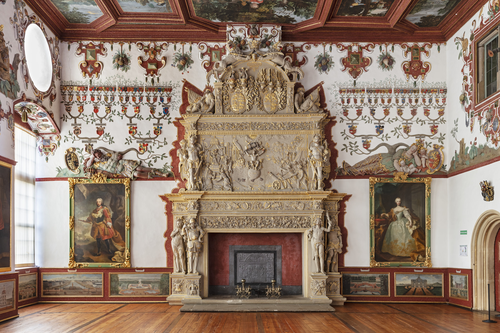
\includegraphics{section_files/figure-pdf/cell-4-output-2.png}
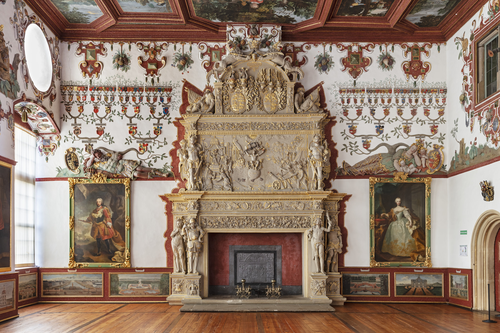
\includegraphics{section_files/figure-pdf/cell-4-output-3.png}

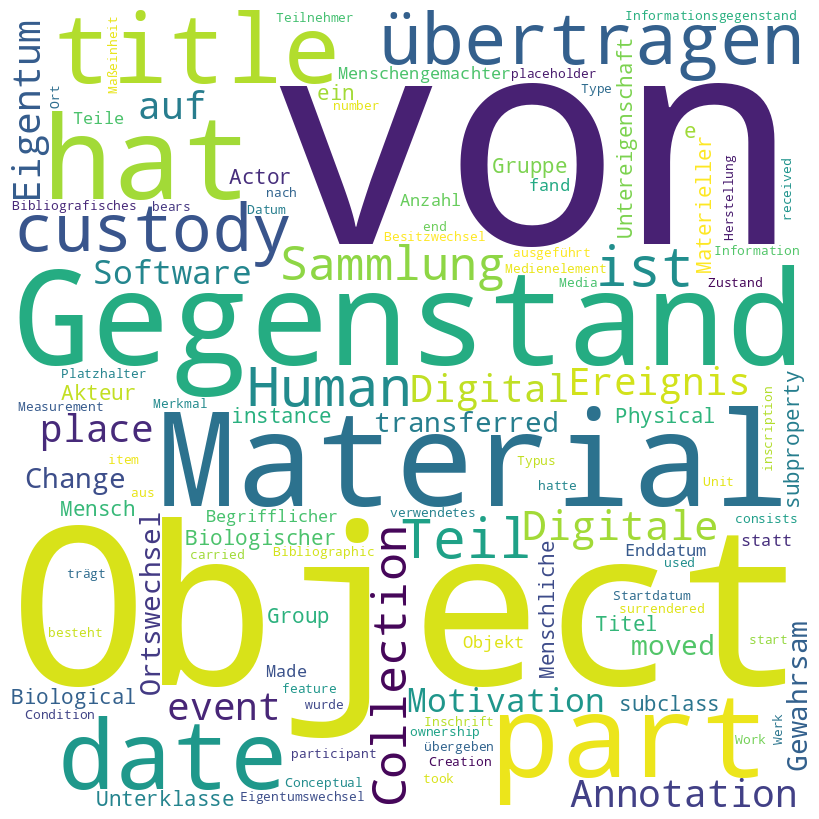
\includegraphics{section_files/figure-pdf/cell-5-output-1.png}


\backmatter

\end{document}
